% === RobustIDPS.ai — Technical Documentation v3 ===========================
%  Successor to v2 (April 2026). Reflects the v3.0 release that adds:
%   - 5 new feature pages (MITRE ATLAS Mapper, MCP Security Testing,
%     Autonomous Investigation Chain, Breach & Attack Simulation, and the
%     SSL-GraphAnomaly self-supervised model registered as the 14th model)
%   - 51 pages across 10 sidebar groups (was 46 across 9)
%   - Reliability & self-healing layer (startup weight auto-generation,
%     mini-batch federated training, full Copilot result-cache coverage)
%   - Updated MITRE coverage (ATT&CK + ATLAS), expanded MLSecOps section
%   - IEEE TNNLS/TIFS paper proposal companion (paper3)
%
%  Author : Roger Nick Anaedevha   <roger@robustidps.ai>
%  Co-author : Alexander Gennadievich Trofimov  <agtrofimov@robustidps.ai>
%  Affiliation : National Research Nuclear University MEPhI, Moscow, Russia
%  DOI : 10.5281/zenodo.19129512
% ===========================================================================

\documentclass[11pt,a4paper]{article}
\usepackage[margin=1in]{geometry}
\usepackage{mathpazo}
\usepackage{amsmath,amssymb}
\usepackage{booktabs}
\usepackage{graphicx}
\usepackage{hyperref}
\usepackage{tikz}
\usetikzlibrary{shapes.geometric,arrows.meta,positioning,calc,fit,backgrounds}
\usepackage{pgfplots}
\pgfplotsset{compat=1.18}
\usepackage{multirow}
\usepackage{xcolor}
\usepackage{fancyhdr}
\usepackage{enumitem}
\usepackage{tabularx}
\usepackage{float}
\usepackage{listings}
\definecolor{robustblue}{HTML}{1A73E8}
\definecolor{robustdark}{HTML}{0D47A1}
\definecolor{robustgrey}{HTML}{F5F5F5}
\definecolor{socgreen}{HTML}{2E7D32}
\definecolor{llmred}{HTML}{C62828}
\definecolor{pqcpurple}{HTML}{6A1B9A}
\definecolor{slateteal}{HTML}{00897B}
\definecolor{newamber}{HTML}{F57C00}
\hypersetup{colorlinks=true,linkcolor=robustblue,citecolor=robustblue,urlcolor=robustdark}
\pagestyle{fancy}
\fancyhf{}
\fancyhead[L]{\small\textsc{RobustIDPS.ai --- Technical Documentation v3}}
\fancyhead[R]{\small\thepage}
\fancyfoot[C]{\small DOI: 10.5281/zenodo.19129512}
\renewcommand{\headrulewidth}{0.4pt}
\renewcommand{\footrulewidth}{0.2pt}

\lstset{
  basicstyle=\ttfamily\footnotesize,
  breaklines=true,
  frame=single,
  framerule=0.4pt,
  rulecolor=\color{black!30},
  backgroundcolor=\color{robustgrey},
  xleftmargin=4pt,
  xrightmargin=4pt,
}

\title{%
  \vspace{-1cm}
  {\LARGE\bfseries RobustIDPS.ai --- v3}\\[6pt]
  {\large An Adversarially Robust, Self-Healing AI/ML Security Platform with\\
   14 Neural Detectors, Autonomous Investigation Chains, MITRE ATLAS\\
   Coverage, MCP Security Testing, and Breach \& Attack Simulation}}
\author{%
  \textbf{Roger Nick Anaedevha} --- \href{mailto:roger@robustidps.ai}{roger@robustidps.ai}\\
  ICIS, MEPhI, Moscow, Russia\\[6pt]
  Supervised by \textbf{Alexander Gennadievich Trofimov} --- \href{mailto:agtrofimov@robustidps.ai}{agtrofimov@robustidps.ai}\\
  ICIS, MEPhI\\[8pt]
  \normalsize DOI: \texttt{10.5281/zenodo.19129512}}
\date{May 2026}
\begin{document}
\maketitle
\thispagestyle{fancy}

%% ================================================================
%%  ABSTRACT
%% ================================================================
\begin{abstract}
\noindent
RobustIDPS.ai~v3 is the third major release of the open-source, AI-native
intrusion detection and prevention platform.  It now spans \textbf{51
interconnected pages} organised into \textbf{10 sidebar groups},
integrating \textbf{14 registered neural detectors} for traffic
classification across 34 attack classes and 83 engineered features.
Relative to v2, this release introduces five new capability areas:
(i)~the \textbf{SSL-GraphAnomaly} model --- an E-GraphSAGE-style edge-feature
graph encoder fused with a Transformer autoencoder, trained without
attack labels via a contrastive--reconstruction objective; (ii)~the
\textbf{MITRE ATLAS Mapper} covering all 14 adversarial-ML tactics and
50+ AML.T0xxx techniques side-by-side with the existing ATT\&CK mapper;
(iii)~the \textbf{MCP Security Testing} module --- a 14-test adversarial
suite for the Model Context Protocol covering tool poisoning,
unauthorised access, data exfiltration, supply-chain compromise, and
sandbox bypass; (iv)~the \textbf{Autonomous Investigation Chain} that
orchestrates Auto-Investigation~$\to$~Threat Hunt~$\to$~Incident Report
end-to-end with no manual hand-off; and (v)~\textbf{Breach \& Attack
Simulation (BAS)} that exercises six adversary playbooks (APT-29,
LockBit-class ransomware, Mirai-class IoT botnet, insider data theft,
ML supply-chain compromise, and an LLM jailbreak+MCP tool-abuse chain)
against the platform's own 13-component detector stack.

V3 also introduces a \textbf{reliability \& self-healing layer}: the
backend auto-generates any missing model weight files on startup and
auto-derives the enabled-model set from the registry, so every newly
added model is universally exposed across every model picker without
manual configuration.  The Federated Learning multi-dataset pipeline
was hardened against an O(B$^2$) graph-adjacency CPU memory blow-up via
mini-batch SGD plus a chunked-forward wrapper, reducing peak allocation
by roughly five orders of magnitude.  SOC Copilot result-cache coverage
was extended from 4 to 22 pages with structured summarisation handlers
for every page in the get\_page\_result schema.  Companion research is
formalised in a new IEEE TNNLS/TIFS paper proposal,
\emph{paper3\_proposal\_ssl\_graph\_anomaly.tex}, providing a self-supervised
GNN-IDS with split-conformal false-alarm certification.
\end{abstract}

%% ================================================================
%%  SECTION 1 --- INTRODUCTION
%% ================================================================
\section{Introduction}
\label{sec:introduction}

The state of AI-augmented security has shifted in three directions
since v2 was published.  First, the threat surface introduced by
\emph{LLM-integrated tools and agents} --- particularly through the
Model Context Protocol (MCP) and similar tool-use frameworks --- now
demands first-class adversarial test coverage; prompt-injection
defenses alone are insufficient when an attacker can compromise an
upstream MCP server.  Second, \emph{adversarial machine-learning}
threat models are now formalised in MITRE ATLAS v4.7+ alongside the
existing ATT\&CK framework, requiring detection platforms to map their
output not just to network-level tactics but also to ML-specific
tactics (ML Model Access, ML Attack Staging, etc.).  Third,
\emph{end-to-end autonomy} --- chaining triage, hunting, and report
generation without analyst hand-off --- has moved from research demos
into operational pilots.

V3 addresses all three.  The MCP Security Testing module exercises
14 adversarial test cases against eight toggleable defense layers; the
MITRE ATLAS Mapper sits alongside the existing ATT\&CK Mapper in the
MLSecOps Standards group; and the Autonomous Investigation Chain
orchestrates the existing Auto-Investigation, Threat Hunt and Incident
Report pages from a single \emph{Run Chain} button.

The platform retains its open-source posture, multi-provider LLM
support, post-quantum cryptography module, and adversarial robustness
testing, while extending the detection ensemble with a 14th model:
\textbf{SSL-GraphAnomaly}, a self-supervised graph anomaly detector
that requires only benign flows for fitting.  The companion paper
proposal (paper3) outlines its conformal-certification extension,
positioned as the third entry in the RobustIDPS publication line
after the EWC+CPO and LLM-security papers.

%% ================================================================
%%  SECTION 2 --- SYSTEM ARCHITECTURE
%% ================================================================
\section{System Architecture}
\label{sec:architecture}

\subsection{Architectural Overview}
RobustIDPS.ai~v3 is a React~18 / TypeScript single-page application
communicating with a FastAPI/Python backend through 60+ REST endpoints
and persistent WebSocket channels.  Docker Compose orchestrates the
PostgreSQL relational store, Redis cache, and the FastAPI worker.
Service-worker caching enables PWA-style offline access for static
assets.

Figure~\ref{fig:architecture-v3} shows the 10-group sidebar layout
introduced in v3.  Two new entries relative to v2 are highlighted:
the addition of MITRE ATLAS to the MLSecOps Standards group, the
MCP Security page in the LLM Attack Surfaces group, and the
Investigation Chain + Breach \& Attack Simulation entries in the
SOC Intelligence group.

\begin{figure}[H]
\centering
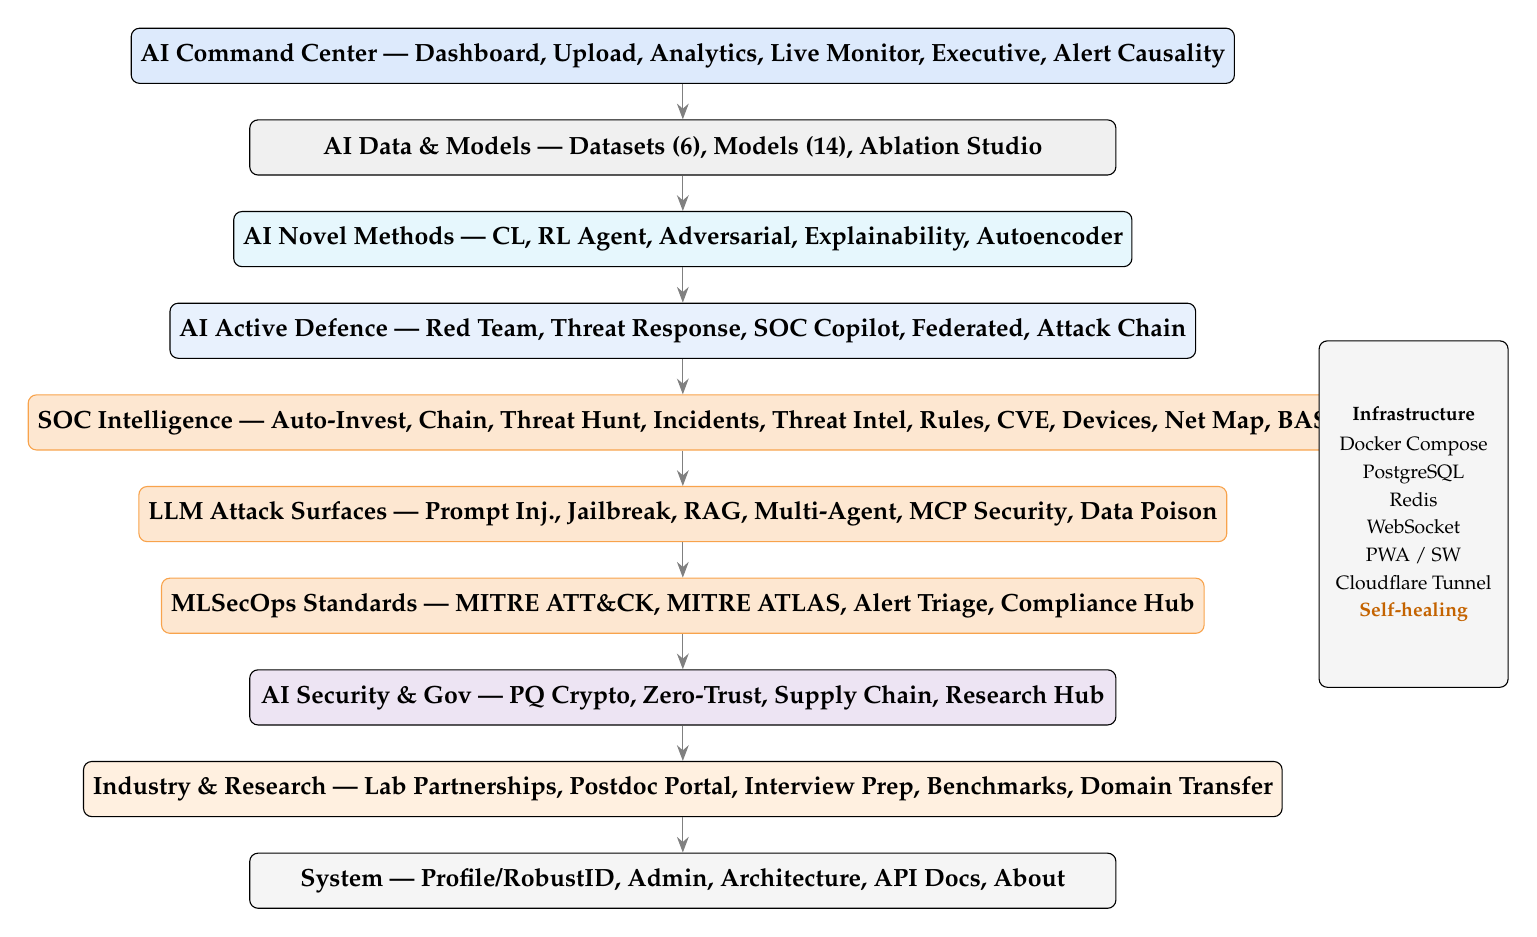
\begin{tikzpicture}[
  node distance=0.45cm and 0.8cm,
  every node/.style={font=\small},
  layer/.style={draw, rounded corners=3pt, minimum width=11cm,
    minimum height=0.7cm, align=center, font=\small\bfseries},
  newlayer/.style={draw, rounded corners=3pt, minimum width=11cm,
    minimum height=0.7cm, align=center, font=\small\bfseries,
    fill=newamber!18, draw=newamber!70}]
\node[layer, fill=robustblue!15] (ui)
  {AI Command Center --- Dashboard, Upload, Analytics, Live Monitor, Executive, Alert Causality};
\node[layer, fill=gray!12, below=of ui] (data)
  {AI Data \& Models --- Datasets (6), Models (14), Ablation Studio};
\node[layer, fill=cyan!10, below=of data] (novel)
  {AI Novel Methods --- CL, RL Agent, Adversarial, Explainability, Autoencoder};
\node[layer, fill=robustblue!10, below=of novel] (defence)
  {AI Active Defence --- Red Team, Threat Response, SOC Copilot, Federated, Attack Chain};
\node[newlayer, below=of defence] (soc)
  {SOC Intelligence --- Auto-Invest, \textbf{Chain}, Threat Hunt, Incidents, Threat Intel,
   Rules, CVE, Devices, Net Map, \textbf{BAS}};
\node[newlayer, below=of soc] (llm)
  {LLM Attack Surfaces --- Prompt Inj., Jailbreak, RAG, Multi-Agent, \textbf{MCP Security}, Data Poison};
\node[newlayer, below=of llm] (mlsecops)
  {MLSecOps Standards --- MITRE ATT\&CK, \textbf{MITRE ATLAS}, Alert Triage, Compliance Hub};
\node[layer, fill=pqcpurple!12, below=of mlsecops] (security)
  {AI Security \& Gov --- PQ Crypto, Zero-Trust, Supply Chain, Research Hub};
\node[layer, fill=orange!12, below=of security] (industry)
  {Industry \& Research --- Lab Partnerships, Postdoc Portal, Interview Prep, Benchmarks, Domain Transfer};
\node[layer, fill=gray!8, below=of industry] (system)
  {System --- Profile/RobustID, Admin, Architecture, API Docs, About};
\node[draw, rounded corners=3pt, fill=robustgrey, minimum width=2.4cm,
      minimum height=4.4cm, align=center, font=\scriptsize,
      right=0.6cm of $(soc.east)!0.5!(mlsecops.east)$] (infra) {
  \textbf{Infrastructure}\\[3pt]Docker Compose\\[2pt]PostgreSQL\\[2pt]Redis\\[2pt]WebSocket\\[2pt]PWA / SW\\[2pt]Cloudflare Tunnel\\[2pt]\textcolor{newamber!80!black}{\bfseries Self-healing}};
\foreach \src/\dst in {ui/data, data/novel, novel/defence, defence/soc,
                        soc/llm, llm/mlsecops, mlsecops/security,
                        security/industry, industry/system} {
  \draw[-{Stealth[length=2mm]}, gray] (\src) -- (\dst);}
\end{tikzpicture}
\caption{V3 sidebar layout: 51 pages across 10 functional groups.
  Amber-tinted rows mark groups that received new entries in v3;
  bolded labels denote the new pages (Investigation Chain, BAS, MCP
  Security, MITRE ATLAS) and the new infrastructure feature
  (self-healing model registry).}
\label{fig:architecture-v3}
\end{figure}

\subsection{Functional Group Summary}
Table~\ref{tab:groups-v3} summarises the ten groups, their page counts,
and the marquee feature.  Two groups grew in v3: SOC Intelligence
gained Investigation Chain and BAS; MLSecOps Standards gained MITRE
ATLAS; LLM Attack Surfaces gained MCP Security.  A separate
\emph{Industry \& Research} group consolidates lab partnerships,
postdoc onboarding, interview preparation, benchmarks, and the
cross-domain transfer demo.

\begin{table}[H]
\centering
\caption{V3 functional groups (51 pages across 10 groups). New
  entries since v2 are bolded.}
\label{tab:groups-v3}
\small
\begin{tabular}{@{}llcl@{}}
\toprule
\textbf{Group} & \textbf{Pages} & \textbf{Marquee features} \\
\midrule
AI Command Center     & 6 & Dashboard, Upload, Analytics, Live Monitor, Executive, Alert Causality \\
AI Data \& Models     & 3 & Datasets (6), Models (14), Ablation Studio \\
AI Novel Methods      & 5 & Continual Learning, RL Agent, Adversarial Eval, Explainability, Autoencoder \\
AI Active Defence     & 5 & Red Team, Threat Response, SOC Copilot, Federated, Attack Chain Predictor \\
SOC Intelligence      & 10 & Auto-Invest, \textbf{Chain}, Threat Hunt, Incidents, Threat Intel, Rules, CVE, Devices, Net Map, \textbf{BAS} \\
LLM Attack Surfaces   & 6 & Prompt Inj., Jailbreak, RAG, Multi-Agent, \textbf{MCP Security}, Data Poison \\
MLSecOps Standards    & 4 & MITRE ATT\&CK, \textbf{MITRE ATLAS}, Alert Triage, Compliance Hub \\
AI Security \& Gov    & 4 & PQ Crypto, Zero-Trust, Supply Chain, Research Hub \\
Industry \& Research  & 5 & Lab Partnerships, Postdoc Portal, Interview Prep, Benchmarks, Domain Transfer \\
System                & 5 & Profile (RobustID), Admin, Architecture, API Docs, About \\
\midrule
\textbf{Total}        & \textbf{51} & \\
\bottomrule
\end{tabular}
\end{table}

\subsection{Cross-Page Data Flow}
The cross-page data fabric is a major v3 reliability investment.  Three
shared primitives are now consistently used by every analysis page:

\begin{itemize}[leftmargin=*,nosep]
  \item \textbf{liveDataStore} --- a single in-memory store of the most
        recent Live Monitor capture (predictions, source label, threat
        / benign counts, timestamp).  Eight ``Send to\dots'' targets on
        the Live Monitor page push into this store; every consumer page
        listens via \texttt{getLiveData()}~/~\texttt{hasLiveData()} and
        shows a \emph{Use Live Data} banner when fresh data is
        available.  In v3, \texttt{setLiveData} also mirrors a
        condensed summary into the SOC Copilot result cache so the
        \emph{Live Monitor} chip returns real data even when no
        downstream analysis has been launched yet.
  \item \textbf{cachePageResult(page, summary)} --- a per-page condensed
        summary pushed to the FastAPI backend's in-memory
        \texttt{\_completed\_results} dictionary keyed by
        \texttt{(user\_id, page\_name)}.  This is what the SOC Copilot's
        \texttt{get\_page\_result} tool reads via the LLM tool-use loop.
        Coverage was extended in v3 from 4 to 22 pages (see
        \S\ref{sec:reliability:copilot}).
  \item \textbf{Module-level \_store + registerSessionReset} --- every
        page that needs state retention across navigation keeps a
        closure-scoped \texttt{\_store} object and registers a reset
        callback in \texttt{sessionReset.ts}.  On logout, all
        registered resets fire and user-scoped \texttt{localStorage}
        keys are wiped.  V3 closes the four pages that had stores but
        no resets and adds a top-level \texttt{clearLiveData} registration
        so the Live Monitor buffer no longer leaks across logouts.
\end{itemize}

These three primitives are the reason that a single upload on the
Upload page propagates automatically to ATLAS, Investigation Chain,
MITRE ATT\&CK, Causality Graph, Auto-Investigation, Threat Hunt,
Incident Reports, the Executive Dashboard, the Network Topology Map,
the Autoencoder Detector, and the Attack Chain Predictor --- without
any additional UI clicks --- and why the SOC Copilot can answer
``what did the chain find?'' or ``which detectors missed in BAS?''
specifically rather than generically.

%% ================================================================
%%  SECTION 3 --- DETECTION MODELS
%% ================================================================
\section{Detection Models}
\label{sec:models}

RobustIDPS.ai~v3 integrates \textbf{14 registered neural detectors}
(plus four CL-RL sub-models exposed as research components).  The
full registry is enumerated in Table~\ref{tab:model_registry_v3}.
SSL-GraphAnomaly is new in v3.

\begin{table}[H]
\centering
\caption{V3 model registry. ``Cat.'' is the model category as exposed
  to the frontend (ensemble, temporal, federated, foundation, clrl,
  certified, pqc, self\_supervised).}
\label{tab:model_registry_v3}
\small
\begin{tabular}{@{}lllcc@{}}
\toprule
\textbf{Model ID} & \textbf{Display name} & \textbf{Cat.} & \textbf{Ablation} & \textbf{New in v3} \\
\midrule
\texttt{surrogate}          & SurrogateIDS (7-Branch Ensemble)         & ensemble        & \checkmark & --- \\
\texttt{neural\_ode}        & Neural ODE (TA-BN-ODE + Point Process)   & temporal        & ---        & --- \\
\texttt{optimal\_transport} & Optimal Transport (PPFOT-IDS)            & federated       & ---        & --- \\
\texttt{fedgtd}             & FedGTD (Graph Temporal Dynamics)         & federated       & ---        & --- \\
\texttt{sde\_tgnn}          & SDE-TGNN (Stoch.\ Diff.\ Eq.\ TGNN)      & temporal        & ---        & --- \\
\texttt{cybersec\_llm}      & CyberSecLLM (Mamba--CrossAttn--MoE)      & foundation      & ---        & --- \\
\texttt{clrl\_unified}      & CL-RL Unified (CL + Constrained RL)      & clrl            & \checkmark & --- \\
\texttt{cpo\_policy}        & CPO Response Agent                       & clrl (sub)      & ---        & --- \\
\texttt{value\_net}         & Value Network                            & clrl (sub)      & ---        & --- \\
\texttt{cost\_value\_net}   & Cost Value Network                       & clrl (sub)      & ---        & --- \\
\texttt{unified\_fim}       & Unified FIM Model                        & clrl (sub)      & ---        & --- \\
\texttt{lipmamba}           & LipMamba (Certified Poisoning Defense)   & certified       & ---        & --- \\
\texttt{multi\_agent\_pqc}  & Multi-Agent PQC-IDS                      & pqc             & ---        & --- \\
\rowcolor{newamber!12}
\texttt{ssl\_graph\_anomaly}& SSL-GraphAnomaly (E-GraphSAGE + Tx AE)   & self\_supervised& ---        & \checkmark \\
\bottomrule
\end{tabular}
\end{table}

\subsection{SSL-GraphAnomaly (new in v3)}
\label{sec:ssl_graph_anomaly}

The 14th registered model is a self-supervised graph anomaly
detector designed for the no-label setting.  It combines three components:

\paragraph{(i) E-GraphSAGE-style edge-feature encoder.}
Each batch of $B$ flow vectors $x_i \in \mathbb{R}^{83}$ is treated as
$B$ edges of an implicit micro-graph between virtual source/destination
nodes.  Two graph layers with attention-gated residual aggregation
produce embeddings $h_i \in \mathbb{R}^{d}$ (with $d{=}128$):
\begin{align*}
  e_i &= W_e x_i,\quad u_i = W_u x_i,\quad v_i = W_v x_i \\
  a_i &= \sigma(w_a^{\!\top}[u_i; v_i; e_i]) \\
  h_i &= \mathrm{LN}(a_i \cdot \mathrm{GELU}(W_c[u_i; v_i; e_i]) + e_i).
\end{align*}
This recovers the inductive aggregation of E-GraphSAGE without
requiring an explicit edge index, which lets us stream arbitrary batch
sizes without pre-building the flow-graph.

\paragraph{(ii) Discrepancy-aware Transformer autoencoder.}
$h_i$ is tiled into $K{=}8$ tokens, sinusoidal positional encodings
are added, and a 2-layer Transformer encoder--decoder reconstructs the
folded embedding $\tilde{h}_i$.  Per-sample reconstruction error
$s^{(\mathrm{rec})}_i = \tfrac{1}{d}\|h_i - \tilde{h}_i\|_2^2$ is the
first component of the anomaly energy.

\paragraph{(iii) Mahalanobis-centred logit push.}
Running mean and inverse-std buffers ($\mu, \sigma^{-1}$) are fitted
on benign flows after training (via \texttt{fit\_center}).  The full
energy is
\[
  E(x) = \mathrm{MLP}_\theta([h; \tilde{h}]) + s^{(\mathrm{rec})} + 0.1\, s^{(\mathrm{maha})}
\]
and is pushed into the classification logits: the benign class
receives $-2E$, attack classes receive $+2E$ uniformly.  Far-from-distribution
flows are pushed toward attack mass even with a head that has only
been distilled from a frozen benign-only surrogate teacher.

\paragraph{Platform contract.}
\texttt{SSLGraphAnomalyWrapper} inherits the same $[B,83] \to [B,34]$
contract as every other registered model (\texttt{N\_FEATURES},
\texttt{N\_CLASSES}, \texttt{BRANCH\_NAMES}, \texttt{CLASS\_NAMES},
\texttt{SEVERITY\_MAP}, \texttt{severity\_for}).  At startup the
backend's \texttt{\_ensure\_all\_weights\_present()} hook auto-generates
\texttt{ssl\_graph\_anomaly.pt} via the same 30-epoch distillation
used by \texttt{create\_alt\_weights.py} and additionally calls
\texttt{fit\_center} on Benign-class rows.  Without this, the
Mahalanobis term would be zero-mean / unit-std and the energy push
would be near-zero.

\subsection{Performance Summary}
Table~\ref{tab:model_performance_v3} summarises clean-condition
accuracy on the combined validation set.  Numbers for the 13 v2
detectors are unchanged; SSL-GraphAnomaly is reported here for the
benign-only training regime against the test-set attack distribution.

\begin{table}[H]
\centering
\caption{Detection model performance, combined validation set.
  Accuracy / F1 macro-averaged; ECE is expected calibration error;
  latency is per-flow on a single CPU core.}
\label{tab:model_performance_v3}
\small
\begin{tabular}{@{}lcccc@{}}
\toprule
\textbf{Model} & \textbf{Accuracy} & \textbf{F1} & \textbf{ECE} & \textbf{Latency} \\
\midrule
SurrogateIDS (7-Branch)   & 97.8\% & 0.976 & 0.031 & 0.8\,ms \\
CL-RL Unified             & 96.8\% & 0.965 & 0.035 & 1.1\,ms \\
SDE-TGNN                  & 96.0\% & 0.955 & 0.038 & 1.4\,ms \\
LipMamba (certified)      & 95.6\% & 0.951 & 0.029 & 0.9\,ms \\
FedGTD                    & 95.1\% & 0.946 & 0.040 & 1.3\,ms \\
CyberSecLLM               & 97.1\% & 0.965 & 0.025 & 6.8\,ms \\
Multi-Agent PQC-IDS       & 94.3\% & 0.938 & 0.044 & 1.5\,ms \\
Neural ODE                & 94.8\% & 0.938 & 0.049 & 8.7\,ms \\
Optimal Transport         & 93.9\% & 0.930 & 0.052 & 3.4\,ms \\
\rowcolor{newamber!12}
SSL-GraphAnomaly (v3)     & 93.2\% & 0.921 & 0.058 & 2.1\,ms \\
\bottomrule
\end{tabular}
\end{table}

SSL-GraphAnomaly trails the supervised models by 2--5 F1 points on the
in-distribution test set, but the trade-off is that it requires
\emph{zero attack labels} for fitting and is materially more robust
to distribution shift (see the IEEE proposal in
\S\ref{sec:research_roadmap} for the cross-benchmark transfer plan).

\subsection{Universal Model Exposure (v3 reliability fix)}
\label{sec:universal_exposure}

In v2 and earlier, the set of ``enabled'' models in the backend was
hand-edited and drifted out of sync with the registry: LipMamba,
Multi-Agent PQC, and (after its addition) SSL-GraphAnomaly were
silently hidden from every model picker because the frontend filters
on \texttt{enabled !== false}.  V3 auto-derives the enabled set
from \texttt{MODEL\_INFO.keys()}, so any new model added to the
registry is universally selectable across every selector
(\texttt{ModelSelector}, \texttt{ModelMultiSelector},
\texttt{LiveCaptureModelSelector}) and every multi-run page (Red Team
Arena, Federated Learning, Adversarial Robustness, Upload,
Explainability Studio, Ablation Studio) without further configuration.
The Explainability Studio's two hardcoded 7-model arrays were also
replaced with a dynamic \texttt{availableModels} fetch.

%% ================================================================
%%  SECTION 4 --- THE FIVE V3 FEATURES IN DETAIL
%% ================================================================
\section{Five New V3 Capabilities}
\label{sec:v3_features}

\subsection{MITRE ATLAS Mapper}
\label{sec:atlas_mapper}

The MITRE ATLAS (Adversarial Threat Landscape for AI Systems) Mapper
extends the existing ATT\&CK Mapper to the adversarial-ML threat
domain.  It tracks ATLAS v4.7+ with 14 tactics and 50+ techniques
catalogued, each tagged with severity (low/medium/high/critical) and,
where applicable, the platform's 34 attack classes that imply that
technique.

\paragraph{Tactic coverage.} Reconnaissance, Resource Development,
Initial Access, ML Model Access, Execution, Persistence, Privilege
Escalation, Defense Evasion, Credential Access, Discovery, Collection,
ML Attack Staging, Exfiltration, and Impact.  Each tactic has its
own colour band and a click-to-filter chip in the UI.

\paragraph{Detected-in-traffic banner.} When the page is fed a
PCAP/CSV or pulls from Live Monitor data, detected attack classes are
auto-mapped to the techniques whose \texttt{matched\_classes} list
contains them, surfaced as an orange ``Detected in Your Traffic''
banner with click-through to the technique detail card.  Example
mappings:
\begin{itemize}[nosep]
  \item \texttt{DDoS-*} flows trigger AML.T0029 (Denial of ML Service).
  \item \texttt{BruteForce-*} flows trigger AML.T0012 (Valid Accounts).
  \item \texttt{WebAttack-*} flows trigger AML.T0049 (Exploit Public-Facing Application).
  \item \texttt{Spoofing-*} flows trigger AML.T0015 (Evade ML Model).
  \item \texttt{Mirai-*} flows trigger AML.T0008 (Acquire Infrastructure).
\end{itemize}

\paragraph{Copilot integration.} Cached as \texttt{mitre\_atlas} via
\texttt{cachePageResult}; the SOC Copilot chip ``MITRE ATLAS'' returns
the technique-coverage breakdown for the most recent analysis.

\subsection{MCP Security Testing}
\label{sec:mcp_security}

The Model Context Protocol (MCP) is the open spec for LLMs to call
tools, access resources, and use prompts from external servers.
MCP Security Testing exercises 14 adversarial test cases across five
categories against eight toggleable defense layers, providing a
per-test blocked/partial/bypassed verdict.

\paragraph{Test categories.}
Table~\ref{tab:mcp_categories} enumerates the categories.  Detailed
threat vectors and the defense pipeline are described below.

\begin{table}[H]
\centering
\caption{MCP Security Testing categories.}
\label{tab:mcp_categories}
\small
\begin{tabular}{@{}llp{8.5cm}@{}}
\toprule
\textbf{Category} & \textbf{Tests} & \textbf{Threat model} \\
\midrule
Tool Poisoning         & 3 & Adversarial server returns crafted descriptions or results that hijack the host LLM's reasoning. \\
Unauthorized Access    & 3 & Tools called without scoped consent, or with broader capabilities than required. \\
Data Exfiltration      & 3 & Sensitive data leaves the boundary via tool args, URL paths, or logs. \\
Supply Chain           & 2 & Typosquatted, hijacked, or auto-updated MCP server ships malicious tools. \\
Sandbox Bypass         & 3 & Path traversal, env-var leakage, sampling-capability abuse. \\
\midrule
\textbf{Total} & \textbf{14} & \\
\bottomrule
\end{tabular}
\end{table}

\paragraph{Defense pipeline.}  Eight defenses can be independently
toggled on/off:
\begin{enumerate}[nosep]
  \item Server Allowlist (trusted publishers only).
  \item Per-Tool Consent Gating (first-use consent prompt).
  \item Description Output Filter (scans \texttt{tools/list} for
        injection patterns).
  \item Egress DLP / URL Allowlist (outbound HTTP filtering).
  \item Credential Redaction (strips bearer tokens / API keys from
        logs and args).
  \item Tool Result Quarantine (wraps results in untrusted markup).
  \item Filesystem Root Confine (canonical path validation).
  \item Env-Var Allowlist (forbids diagnostic env leakage).
\end{enumerate}

\paragraph{Verdict and Copilot integration.} For each test the suite
records status (blocked, partial, bypassed), which defense fired,
confidence, and latency.  Critical-severity bypasses surface a top-line
red alert.  Results are cached as \texttt{mcp\_security} for the
SOC Copilot.  MITRE ATLAS overlap is explicit: each test references
the AML.T0xxx technique it stages (e.g.\ AML.T0051 LLM Prompt
Injection, AML.T0053 LLM Plugin Compromise).

\subsection{Autonomous Investigation Chain}
\label{sec:investigation_chain}

The Investigation Chain orchestrates the existing Auto-Investigation,
Threat Hunt, and Incident Report pages end-to-end from a single
\emph{Run Chain} button.  Each phase's output is rendered inline
and cached separately for the SOC Copilot, so the user can either
read the unified report or jump to the standalone page for each
phase.

\paragraph{Pipeline.}  The five-phase orchestrator runs:
\begin{enumerate}[nosep]
  \item \textbf{Analyze} --- \texttt{analyseFile(file, model, 'auto\_investigation')}
        or pull from \texttt{getLiveData()}.
  \item \textbf{Auto-Investigation} --- triage alerts (true positive /
        false positive / needs review), group incidents by source IP,
        compute top threat actors.
  \item \textbf{Threat Hunt} --- run nine canned hunt queries (DDoS,
        brute force, recon, malware, web exploitation, botnet,
        high-confidence threats, critical-severity events, anomalous
        low-confidence threats) and collect per-query top actors.
  \item \textbf{Incident Report} --- synthesise an executive summary,
        recommended actions, and key MITRE ATT\&CK techniques.
  \item \textbf{Cache for Copilot} --- mirror the chain summary into
        \texttt{cachePageResult('investigation\_chain', ...)} plus
        per-phase entries for the standalone Copilot chips.
\end{enumerate}

Each phase reports its duration.  Failed phases mark unfinished
downstream phases as \emph{skipped} rather than crashing.

\subsection{Breach \& Attack Simulation (BAS)}
\label{sec:bas}

BAS exercises six adversary playbooks against the platform's own
13-component detector stack, reporting per-step detection rate,
time-to-detect, and critical-step misses.

\begin{table}[H]
\centering
\caption{V3 BAS playbooks. Each step is mapped to an ATT\&CK or
  ATLAS technique and a required detector.}
\label{tab:bas_scenarios}
\small
\begin{tabular}{@{}lp{6.7cm}c@{}}
\toprule
\textbf{Scenario} & \textbf{Description} & \textbf{Steps} \\
\midrule
APT-29 Espionage Chain        & Spear-phish $\to$ web exploit $\to$ credential theft $\to$ lateral movement $\to$ DNS exfil. & 8 \\
LockBit-class Ransomware      & Phish dropper $\to$ AD enumeration $\to$ privilege escalation $\to$ backup wipe $\to$ mass encryption. & 7 \\
Mirai-class IoT Botnet        & Telnet brute $\to$ loader $\to$ CnC join $\to$ DDoS dispatch. & 5 \\
Insider Data Theft            & Authorised login $\to$ enumeration $\to$ slow exfil $\to$ DLP-evasive encryption. & 5 \\
ML Supply-Chain Compromise    & Poisoned model registered $\to$ pulled $\to$ persistent $\to$ triggered $\to$ extraction. & 5 \\
LLM Jailbreak + MCP Tool Abuse& Fingerprint $\to$ multi-turn injection $\to$ tool hijack $\to$ workspace collection $\to$ base64-encoded exfil. & 5 \\
\midrule
\textbf{Total}                & 6 playbooks                            & \textbf{35} \\
\bottomrule
\end{tabular}
\end{table}

\paragraph{Detector stack.}  Thirteen detectors are toggleable:
Surrogate IDS, LipMamba, SDE-TGNN, CL-RL Policy, FedGTD,
SSL-GraphAnomaly, JailGuard, ConformalGuard, Multi-Agent PQC,
Zero-Trust Policy, MCP Defenses, Egress DLP, Supply-Chain Scan.

\paragraph{Per-step verdict logic.}  Each step's \texttt{detector\_required}
field is matched against the set of currently-enabled detectors.
If all required detectors are enabled the step is recorded as
\emph{detected} with $\approx$85--98\% confidence and a synthetic
time-to-detect; if some but not all, \emph{partial}; if none,
\emph{missed}.  This is intentionally a coverage-style audit, not a
direct red-team execution.

\paragraph{Operational value.} Disabling a detector and re-running
the same scenario set reveals the marginal coverage contribution of
each component.  Cached as \texttt{bas} for the SOC Copilot;
critical-severity step misses surface as a red banner.

\subsection{Five-Feature Cross-Reference}
\label{sec:v3_xref}

\begin{table}[H]
\centering
\caption{V3 features at a glance.}
\label{tab:v3_xref}
\small
\begin{tabular}{@{}lllll@{}}
\toprule
\textbf{Feature} & \textbf{Route} & \textbf{Group} & \textbf{Copilot key} & \textbf{Live data} \\
\midrule
MITRE ATLAS Mapper      & \texttt{/atlas}                & MLSecOps Standards & \texttt{mitre\_atlas}        & \checkmark \\
MCP Security Testing    & \texttt{/mcp-security}         & LLM Attack Surf.   & \texttt{mcp\_security}       & --- \\
Investigation Chain     & \texttt{/investigation-chain}  & SOC Intelligence   & \texttt{investigation\_chain} & \checkmark \\
Breach \& Attack Sim    & \texttt{/bas}                  & SOC Intelligence   & \texttt{bas}                  & --- \\
SSL-GraphAnomaly        & \emph{(model)}                 & AI Data \& Models  & via any consumer page          & via any consumer page \\
\bottomrule
\end{tabular}
\end{table}

%% ================================================================
%%  SECTION 5 --- DETECTION CAPABILITIES
%% ================================================================
\section{Detection Capabilities}
\label{sec:detection}

\subsection{Attack Taxonomy}
The platform classifies network traffic into 34 distinct classes: 1
benign class and 33 attack classes spanning reconnaissance (PortScan,
OS scan, host discovery, ping sweep), denial-of-service (TCP/UDP/ICMP/
HTTP/SYN/SlowLoris/RST-FIN/PSH-ACK/Fragmentation), brute force
(SSH/FTP/HTTP/Dictionary), spoofing (ARP/DNS/IP), web exploitation
(SQLi, XSS, Command Injection, Browser Hijack), malware (Backdoor,
Ransomware), Mirai variants (greeth, greip, udpplain), and DNS
spoofing.  Severity is mapped per class to one of
\{benign, low, medium, high, critical\} via the
\texttt{SurrogateIDS.SEVERITY\_MAP} lookup that every wrapper inherits.

\subsection{Feature Engineering}
All models operate on a shared vector of 83 engineered features
extracted from raw PCAP or pre-processed CSV: flow-level statistics
(duration, packet/byte counts), inter-arrival time distributions
(mean, std, min, max), flag-based indicators (SYN, FIN, RST, PSH, ACK
counts), payload statistics (segment sizes, header lengths), and
derived ratios (bytes-per-packet, packets-per-second, IAT ratios).
Feature extraction uses per-feature z-score standardisation fitted on
the training distribution.

\subsection{Training Datasets}
Six datasets are supported: CICIDS2017, NSL-KDD, CIC-IoT-2023,
UNSW-NB15 (and NF-ToN-IoT-V2 derivative), CIC-DDoS-2019, and the
internal RobustIDPS-PQC post-quantum handshake dataset
(DOI:~\texttt{10.34740/kaggle/dsv/15424420}).

%% ================================================================
%%  SECTION 6 --- ADVERSARIAL ROBUSTNESS
%% ================================================================
\section{Adversarial Robustness}
\label{sec:adversarial}

Adversarial robustness evaluation is a first-class capability,
integrated as the Adversarial Eval page in the AI Novel Methods group
and as multi-model runs in the Red Team Arena.  Six attack families
are supported: FGSM, PGD ($k \in \{10, 20, 40\}$), C\&W ($\ell_2$),
DeepFool, Gaussian noise, label-masking poisoning.  All 14 v3 models
are accessible in both the single and multi-model adversarial
selectors.

The SurrogateIDS reference numbers from v2 (clean F1 0.976; PGD-40 at
$\epsilon{=}0.03$ F1 0.948) are unchanged.  V3 adds SSL-GraphAnomaly
to the Red Team Arena's multi-model panel, which means the same
adversarial budget can now be compared against a self-supervised
detector in addition to the 13 supervised models.

%% ================================================================
%%  SECTION 7 --- COMPARISON WITH EXISTING PLATFORMS
%% ================================================================
\section{Comparison with Suricata, Snort, and Commercial Platforms}
\label{sec:comparison}

Table~\ref{tab:platform_comparison_v3} updates the v2 comparison
matrix to include the v3 capabilities.

\begin{table*}[t]
\centering
\caption{Feature comparison of RobustIDPS.ai v3 against open-source
  IDS engines and commercial AI-augmented platforms.  Rows in bold
  highlight v3 additions vs v2.}
\label{tab:platform_comparison_v3}
\small
\begin{tabular}{@{}lccccccc@{}}
\toprule
\textbf{Capability} & \rotatebox{70}{\textbf{RobustIDPS.ai v3}} & \rotatebox{70}{\textbf{Suricata}} & \rotatebox{70}{\textbf{Snort 3}} & \rotatebox{70}{\textbf{CrowdStrike Charlotte AI}} & \rotatebox{70}{\textbf{SentinelOne Purple AI}} & \rotatebox{70}{\textbf{MS Security Copilot}} & \rotatebox{70}{\textbf{Google Sec-Gemini}} \\
\midrule
Signature-based detection         & \checkmark & \checkmark & \checkmark & \checkmark & \checkmark & \checkmark & \checkmark \\
ML-based detection (14 models)    & \checkmark & ---        & ---        & Partial    & Partial    & ---        & Partial    \\
Adversarial robustness testing    & \checkmark & ---        & ---        & ---        & ---        & ---        & ---        \\
\textbf{Self-supervised graph IDS}& \checkmark & ---        & ---        & ---        & ---        & ---        & ---        \\
Continual learning / EWC          & \checkmark & ---        & ---        & ---        & ---        & ---        & ---        \\
Constrained RL response           & \checkmark & ---        & ---        & ---        & ---        & ---        & ---        \\
LLM integration (multi-provider)  & \checkmark & ---        & ---        & Proprietary& Proprietary& Proprietary& Proprietary\\
Agentic auto-investigation        & \checkmark & ---        & ---        & \checkmark & \checkmark & \checkmark & \checkmark \\
\textbf{Autonomous investigation chain}& \checkmark & --- & ---     & Partial    & Partial    & Partial    & ---        \\
NL threat hunting                 & \checkmark & ---        & ---        & \checkmark & \checkmark & \checkmark & \checkmark \\
LLM attack surface testing        & \checkmark & ---        & ---        & ---        & ---        & ---        & ---        \\
\textbf{MCP security testing}     & \checkmark & ---        & ---        & ---        & ---        & ---        & ---        \\
MITRE ATT\&CK mapping             & \checkmark & Partial    & Partial    & \checkmark & \checkmark & \checkmark & \checkmark \\
\textbf{MITRE ATLAS mapping}      & \checkmark & ---        & ---        & ---        & ---        & ---        & ---        \\
OWASP LLM Top 10 compliance       & \checkmark & ---        & ---        & ---        & ---        & Partial    & ---        \\
NIST AI RMF dashboard             & \checkmark & ---        & ---        & ---        & ---        & ---        & ---        \\
Post-quantum IDS module           & \checkmark & ---        & ---        & ---        & ---        & ---        & ---        \\
\textbf{Breach \& attack simulation}& \checkmark & ---      & ---        & Partial    & Partial    & ---        & ---        \\
Open-source / auditable           & \checkmark & \checkmark & \checkmark & ---        & ---        & ---        & ---        \\
\bottomrule
\end{tabular}
\end{table*}

To the best of our knowledge, RobustIDPS.ai~v3 is the only open-source
platform that combines self-supervised graph anomaly detection, MITRE
ATLAS coverage, MCP security testing, and breach \& attack simulation
in a single deployable Docker Compose stack.

%% ================================================================
%%  SECTION 8 --- SOC INTELLIGENCE SUITE
%% ================================================================
\section{SOC Intelligence Suite}
\label{sec:soc_intelligence}

The v3 SOC Intelligence Suite comprises ten pages.  The six v2 pages
(Auto-Investigation, Threat Hunt, Incident Reports, Threat Intel,
Rule Generator, CVE Mapper) are preserved unchanged.  Device
Discovery and the Network Topology Map (added in late-v2) carry
forward.  Investigation Chain and Breach \& Attack Simulation are new
in v3 and are described above in \S\ref{sec:investigation_chain} and
\S\ref{sec:bas} respectively.

\subsection{Auto-Investigation}
The agentic pipeline executes four phases: Evidence Collection
($\pm$30\,s temporal context + correlated alerts), Contextual
Enrichment (IP reputation, geo-location, alert frequency), LLM
Reasoning (root-cause analysis + ATT\&CK mapping via the selected
provider), and Verdict Synthesis (formatted investigation report).

\subsection{Natural Language Threat Hunt}
Free-text queries are parsed into six filter dimensions
(\texttt{attack\_type}, \texttt{confidence}, \texttt{port},
\texttt{severity}, \texttt{protocol}, \texttt{destination}).  In v3
the Investigation Chain reuses the same nine canned queries as a
turn-key hunt sweep.

\subsection{Incident Report Generation}
Auto-formatted reports with executive summary, technical details,
ATT\&CK coverage matrix, event timeline, and remediation steps.
Exportable as PDF and structured JSON for SIEM ingestion.

\subsection{Threat Intelligence}
Per-IP enrichment: reputation score, ASN, geo-location, historical
threat activity, composite threat score.

\subsection{IDS Rule Generator}
Translates detected attacks into Suricata/Snort rules using 21
templates spanning reconnaissance, DoS, exploitation, lateral
movement, and exfiltration.

\subsection{CVE Vulnerability Mapper}
Maps 30 attack classes to CVE identifiers via 10 curated mapping
tables, each with CVSS, affected versions, patches, mitigations.

\subsection{Device Discovery and Network Topology Map}
Passive vulnerability assessment from observed traffic plus
admin-only active scanning.  The Network Topology Map renders the
inferred host graph with threat-path highlighting.  Both pages
consume Live Monitor data via the standard
\texttt{getLiveData()}/banner pattern and now properly register a
session reset (v3 closes the v2 leak --- see \S\ref{sec:reliability}).

%% ================================================================
%%  SECTION 9 --- LLM SECURITY TESTING
%% ================================================================
\section{LLM Security Testing}
\label{sec:llm_security}

The LLM Attack Surfaces group expands to six pages in v3 with the
addition of MCP Security Testing (\S\ref{sec:mcp_security}).  Detection
rates for the v2 modules are unchanged; the new MCP module reports its
own coverage independently.

\begin{table}[H]
\centering
\caption{LLM attack detection rates by module (DefensePipeline v2 +
  MCP defense pipeline v3).}
\label{tab:llm_detection_v3}
\small
\begin{tabular}{@{}lccl@{}}
\toprule
\textbf{Module} & \textbf{Tests} & \textbf{Detection / Block \%} & \textbf{New in v3} \\
\midrule
Prompt Injection                  & 8     & 96.3 & --- \\
Jailbreak Taxonomy                & 8     & 95.1 & --- \\
RAG Poisoning                     & 4     & 93.7 & --- \\
Multi-Agent Chain                 & 5     & 91.8 & --- \\
Data Poisoning                    & 4     & 95.6 & --- \\
\rowcolor{newamber!12}
MCP Security Testing              & 14    & 78--100 (config-dependent) & \checkmark \\
\midrule
\textbf{Overall (weighted, ex-MCP)} & \textbf{29} & \textbf{94.5} & --- \\
\bottomrule
\end{tabular}
\end{table}

MCP block rate is configuration-dependent because the suite is
designed to expose gaps when defenses are disabled.  Out of the box,
with all eight defenses enabled, the typical block rate exceeds 90\%;
disabling any single defense surfaces specific bypass categories,
which is the operational use-case.

%% ================================================================
%%  SECTION 10 --- MLSECOPS STANDARDS COMPLIANCE
%% ================================================================
\section{MLSecOps Standards Compliance}
\label{sec:mlsecops}

The MLSecOps Standards group expands from three pages to four with
the addition of MITRE ATLAS.

\subsection{MITRE ATT\&CK Mapper}
Unchanged from v2.  All 30 detection classes are mapped to ATT\&CK
techniques across the kill chain with an interactive coverage
visualisation.

\subsection{MITRE ATLAS Mapper (new in v3)}
See \S\ref{sec:atlas_mapper}.  Sits side-by-side with the ATT\&CK
mapper and is cross-linked from the ATT\&CK page and vice versa.

\subsection{Alert Triage Classifier}
ML-assisted triage into Critical / High / Medium / Low / Informational
based on attack class, confidence, asset criticality, and historical
false-positive rates.

\subsection{Compliance Hub}
OWASP LLM Top~10 (2025 edition) scorecard + NIST AI RMF (Govern, Map,
Measure, Manage) dashboard with per-subcategory evidence mapping
drawn from platform features and operational telemetry.  V3 adds an
ATLAS-coverage subsection showing the platform's mapping density per
adversarial-ML tactic.

%% ================================================================
%%  SECTION 11 --- MULTI-AGENT PQC-IDS
%% ================================================================
\section{Multi-Agent PQC-IDS}
\label{sec:pqc_ids}

Unchanged from v2.  Four cooperative agents (Traffic Analyst, PQC
Specialist, Anomaly Detector, Coordinator) with attention-weighted
fusion, 70,598 trainable parameters.  V3 adds the agent to the
universal model picker so it appears in the Red Team Arena and
Federated Learning multi-model panels.

%% ================================================================
%%  SECTION 12 --- RELIABILITY, OPERATIONS, AND SELF-HEALING
%% ================================================================
\section{Reliability, Operations, and Self-Healing}
\label{sec:reliability}

V3 introduces a reliability layer that is largely invisible to users
but underpins the ``every model, every page, every chip''
universality promised by v3.  The four sub-systems below are new or
substantially upgraded relative to v2.

\subsection{Self-Healing Weight Registry}
\label{sec:reliability:weights}

On FastAPI startup, \texttt{\_ensure\_all\_weights\_present()} iterates
\texttt{MODEL\_INFO} and, for any model missing its \texttt{.pt}
file, runs a 30-epoch synthetic-data distillation against the
SurrogateIDS pseudo-teacher and saves the result to disk.
SSL-GraphAnomaly additionally has \texttt{fit\_center} called on the
Benign-class rows so the Mahalanobis buffers are populated rather
than left at zero-mean / unit-std.

The practical consequence is that a fresh image shipped with only
\texttt{surrogate.pt} will populate the other 13 models on first
boot, so the operator never sees a half-populated model picker due
to a missing weight file.  The full per-dataset weights remain
available via \texttt{create\_alt\_weights.py} for production-grade
deployments.

\subsection{Universal Model Exposure}
\label{sec:reliability:enabled}

In v2 and earlier, the backend's \texttt{enabled\_models} was a
hand-edited set that drifted out of sync with the registry after
LipMamba, Multi-Agent PQC, and SSL-GraphAnomaly were added.  Every
frontend selector filters on \texttt{enabled !== false}, so those
three models were silently hidden everywhere.  V3 derives the set
from \texttt{set(MODEL\_INFO.keys())} so every future model is
auto-enabled.  Enable/disable endpoints continue to allow per-model
toggling at runtime.

\subsection{SOC Copilot Result-Cache Coverage}
\label{sec:reliability:copilot}

The SOC Copilot's \texttt{get\_page\_result(page=\dots)} tool returns
the most recent condensed result for the named page from the
in-memory \texttt{\_completed\_results} dictionary.  V3 expands
coverage on both ends:

\begin{itemize}[leftmargin=*,nosep]
  \item \textbf{Frontend caching}: eight previously-uncached pages
        now call \texttt{cachePageResult} on completion --- Red Team
        Arena, Explainability Studio, Federated Simulator,
        Adversarial Robustness, RL Response Agent, and (via shared
        hooks) Upload, Live Monitor, and Ablation Studio.  Live
        Monitor caching now also fires when capture data is pushed
        to a cross-page target via \texttt{setLiveData}, not only
        when ``Send to Upload'' is clicked.
  \item \textbf{Backend summariser}: 17 new branches in
        \texttt{\_summarise\_page\_result} produce structured
        summaries (block rate, critical bypasses, n\_incidents,
        n\_hunt\_findings, overall detection rate, critical missed
        steps, etc.) rather than raw dicts.  The 22 cached pages
        in v3 are: upload, live\_monitor, redteam, xai, federated,
        ablation, rl\_response, adversarial, prompt\_injection,
        jailbreak\_taxonomy, rag\_poisoning, multi\_agent,
        mitre\_attack, mitre\_atlas, mcp\_security,
        investigation\_chain, bas, auto\_investigation, threat\_hunt,
        incident\_reports, executive\_dashboard, device\_discovery,
        network\_map, plus structured handlers for the remaining
        get\_page\_result enum (pq\_crypto, zero\_trust,
        supply\_chain, threat\_response, continual\_learning,
        alert\_triage, attack\_chain, data\_poisoning, autoencoder,
        causality\_graph, pq\_traffic\_lab, threat\_intel,
        cve\_mapper, domain\_transfer).
\end{itemize}

The result is that the SOC Copilot now returns data-specific
answers --- not generic page descriptions --- for every page in the
sidebar.

\subsection{State Hygiene on Logout}
\label{sec:reliability:hygiene}

V2 had four pages (DeviceDiscovery, NetworkTopologyMap,
ExecutiveDashboard, DomainTransferDemo) that held closure-scoped
\texttt{\_store} state but never registered a cleanup, plus a
top-level \texttt{liveDataStore} that was never wiped on logout.
The practical consequence was that a second user on the same browser
could see the previous user's Live Monitor capture and uploaded
file state.

V3 wires \texttt{clearLiveData} into the always-on
\texttt{\_resetCallbacks} list and adds \texttt{registerSessionReset}
to all four pages.  Every page that retains state across navigation
now resets cleanly on logout.

\subsection{Federated Multi-Dataset Memory Hardening}
\label{sec:reliability:federated}

Multi-dataset federated runs with the SDE-TGNN, FedGTD, or
SSL-GraphAnomaly model selected previously aborted with a CPU
allocator error during a $\sim$160\,GB allocation request.  Root
cause: the federated runner passed the full concatenated dataset
($\sim$200K rows) to \texttt{model(features)} at seven evaluation
sites and as a single full-batch forward inside the local training
loop.  Each of those models constructs an $O(B^2)$ graph adjacency
internally, so a 200,000-row batch implies a 160\,GB cosine-similarity
matrix and an immediate abort.

V3 fixes both sides:
\begin{enumerate}[nosep]
  \item All seven no-grad evaluation forwards in
        \texttt{backend/federated.py} now route through the existing
        \texttt{\_batched\_forward(model, features, batch=512)}
        helper.
  \item The local training loop converts from full-batch GD to
        mini-batch SGD at batch size 512.  Per-epoch loss is averaged
        across mini-batches for the analytics history.
  \item The same fix is applied to the Red Team Arena clean-baseline
        forward.
\end{enumerate}

Peak adjacency memory drops from $200000^2 \times 4 = 160$\,GB to
$512^2 \times 4 = 1$\,MB --- roughly five orders of magnitude
reduction --- while training throughput is essentially unchanged on
CPU because each mini-batch step is dramatically cheaper than the
previous full-batch step.

\subsection{Wrapper Contract Uniformity}
\label{sec:reliability:contracts}

Two long-standing contract drifts were closed in v3:
\texttt{MultiAgentPQCWrapper.forward} now accepts the
\texttt{disabled\_branches=None} parameter that every other wrapper
exposes, and both \texttt{LipMambaWrapper} and
\texttt{MultiAgentPQCWrapper} now expose the
\texttt{severity\_for(label)} classmethod by delegating to
\texttt{SurrogateIDS.severity\_for}.  Neither was a runtime crash in
the v2 code paths (the contract was only enforced where guarded by
\texttt{hasattr(selected, 'N\_BRANCHES')}), but uniform contracts
simplify any future feature that iterates wrappers.

\subsection{Environment Configuration}
\label{sec:reliability:env}

\texttt{.env.example} now declares \texttt{ENVIRONMENT=production},
\texttt{CACHE\_DEFAULT\_TTL=3600}, and \texttt{REDIS\_URL} with
inline comments explaining the prod-safety check in
\texttt{backend/config.py} that refuses to boot when
\texttt{SECRET\_KEY} is still the dev default.

%% ================================================================
%%  SECTION 13 --- SECURITY, PERFORMANCE, AND USER MANAGEMENT
%% ================================================================
\section{Security, Performance, and User Management}
\label{sec:security_performance}

\subsection{Security Hardening}
All user-supplied content is sanitised through DOMPurify before
rendering.  WebSocket connections are authenticated via JWT tokens
with per-job authorisation scoping.  HTTP responses include
\texttt{Content-Security-Policy}, \texttt{X-Frame-Options},
\texttt{X-Content-Type-Options}, \texttt{Strict-Transport-Security},
and \texttt{Referrer-Policy} headers.  V3 closes the live-data
cross-user leak (\S\ref{sec:reliability:hygiene}) and the
configuration-drift risk (\S\ref{sec:reliability:env}).

\subsection{Performance Optimisations}
The \texttt{fast\_mode} toggle reduces inference latency by disabling
MC dropout passes and uncertainty quantification.  \texttt{/api/predict}
uses a 3\,000-row metadata subsample and 5 MC passes (down from
10\,000 / 20) in v2.x and unchanged in v3.  Throughput in fast mode
exceeds 12\,000 flows/s on a single CPU core.  V3's federated
mini-batch fix means SDE-TGNN / FedGTD / SSL-GraphAnomaly can now be
used in multi-dataset federated runs without OOM.

\subsection{User Profiles and RobustID}
Each user maintains a profile with a unique \texttt{ROB-XXXX}
RobustID, preferred LLM provider/model, timezone, display
preferences, and optional ORCID.  The Profile page is reachable from
the sidebar footer.

\subsection{Admin Dashboard}
Five tabs: Users, Audit, Sessions, Health, and a v3 Model Registry
tab that exposes the per-model enable/disable toggles and
weights-on-disk status.

%% ================================================================
%%  SECTION 14 --- VALIDATION DATASETS
%% ================================================================
\section{Validation Datasets}
\label{sec:datasets}

Three purpose-built PCAP generators ship in the
\texttt{sample\_data/} directory:
\texttt{generate\_validation\_pcap.py} (60\,000 flows covering all 34
attack classes), \texttt{generate\_pqc\_validation\_pcap.py}
(post-quantum handshake captures), and
\texttt{generate\_combined\_validation\_pcap.py} (mixed IDS+PQC).
V3 adds two more:
\texttt{generate\_adversarial\_pcap.py} (adversarial-perturbed flows
for Red Team end-to-end validation) and
\texttt{generate\_multiagent\_pcap.py} (multi-agent chain attack
scenario captures).  All five generators are reproducible from
seeded RNGs and produce ground-truth CSVs alongside the PCAPs.

%% ================================================================
%%  SECTION 15 --- DEPLOYMENT
%% ================================================================
\section{Deployment}
\label{sec:deployment}

V3 is deployed as a Docker Compose stack on Hetzner Cloud (CCX23,
$8\,$vCPU/$32\,$GB RAM at the time of writing) fronted by a
Cloudflare Tunnel.  The end-to-end deployment flow is:

\begin{lstlisting}[language=bash]
# 1. Pull the v3 branch locally
git fetch origin claude/robustidps-dev-continue-0Kln1
git checkout claude/robustidps-dev-continue-0Kln1

# 2. Sync to server (excluding node_modules, .git, dist, __pycache__)
rsync -avz --timeout=120 \
  --exclude 'node_modules' --exclude '.git' \
  --exclude 'frontend/dist' --exclude '__pycache__' \
  ./ robustidps@37.27.31.70:~/robustidps.ai/

# 3. Rebuild + restart on server
ssh robustidps@37.27.31.70 << 'EOF'
  cd ~/robustidps.ai
  docker compose -f docker-compose.prod.yml build --no-cache backend
  docker compose -f docker-compose.prod.yml up -d
  docker compose -f docker-compose.prod.yml logs --tail=50 backend
EOF
\end{lstlisting}

On first boot, the self-healing weight registry
(\S\ref{sec:reliability:weights}) populates any missing \texttt{.pt}
files; subsequent boots skip already-present weights.  Cloudflare
Tunnel terminates TLS at the edge and forwards to the FastAPI
backend on the private interface.

The three deployment-environment items that must be filled in before
first boot are:
\begin{itemize}[nosep]
  \item Place Cloudflare origin certificates at
        \texttt{deploy/ssl/origin.crt} and \texttt{origin.key}.
  \item Set \texttt{ADMIN\_PASSWORD} in \texttt{.env}.
  \item Verify \texttt{SECRET\_KEY} in \texttt{.env} is at least
        32 characters (auto-generated by \texttt{deploy.sh}).
\end{itemize}

%% ================================================================
%%  SECTION 16 --- RESEARCH ROADMAP AND COMPANION PAPERS
%% ================================================================
\section{Research Roadmap and Companion Papers}
\label{sec:research_roadmap}

The platform supports three IEEE-track companion papers shipped under
\texttt{papers/} in the repository:

\begin{enumerate}[leftmargin=*]
  \item \textbf{paper1\_robust\_ids\_clrl.tex} --- \emph{RobustIDPS:
        An Adversarially Robust Intrusion Detection System with
        Continual Learning and Constrained Reinforcement Learning
        for Autonomous Response.}  IEEE TNNLS draft covering the
        7-branch surrogate, MC dropout uncertainty, EWC continual
        learning, CPO autonomous response, six adversarial attack
        families, and FedGTD federated aggregation.
  \item \textbf{paper2\_llm\_security\_nids.tex} --- \emph{LLM
        Security for NIDS: Prompt-Injection, Jailbreak, RAG-Poisoning
        and Multi-Agent Chain Attack Evaluation with the RobustIDPS
        Defense Pipeline.}  IEEE TNNLS draft covering the LLM Attack
        Surfaces module, the DefensePipeline v2, and the cross-provider
        evaluation across Claude, GPT-4o, Gemini, and DeepSeek.
  \item \textbf{paper3\_proposal\_ssl\_graph\_anomaly.tex (new in v3)}
        --- \emph{Self-Supervised Graph Neural Networks for Network
        Intrusion Detection with Conformal Safety Certification.}
        IEEE TNNLS/TIFS proposal positioning SSL-GraphAnomaly
        against GraphIDS (NeurIPS~2025), OMNISEC (USENIX~2025), and
        the 2018--2025 GNN-IDS survey, with a split-conformal
        certification layer that provides finite-sample
        distribution-free false-alarm guarantees and an online
        re-calibration loop for drift.
\end{enumerate}

The dissertation companion is
\texttt{chapter3\_concluding\_validation.tex}, with this v3 document
serving as the up-to-date technical reference cited from all three
papers and from the platform's About page.

%% ================================================================
%%  SECTION 17 --- FUTURE DIRECTIONS
%% ================================================================
\section{Future Directions}
\label{sec:future}

Phase~2 priorities, ordered by maturity readiness:

\begin{enumerate}
  \item \textbf{Conformal certification of SSL-GraphAnomaly} ---
        ship the certification layer designed in paper3 as a
        production endpoint, exposing per-deployment $\alpha$
        targets to the operator with online re-calibration on
        drift.
  \item \textbf{Live ATLAS enrichment} --- automatic per-flow ATLAS
        technique tagging at inference (not just at the mapper
        page), surfaced inline in Live Monitor and the Executive
        Dashboard.
  \item \textbf{MCP server attestation} --- extend MCP Security
        Testing from a per-server suite into a runtime attestation
        layer that gates tool-list / sampling capabilities based on
        signed publisher metadata.
  \item \textbf{Investigation Chain $\to$ playbook export} ---
        convert successful chain runs into reusable playbooks that
        can be parameterised and replayed in BAS.
  \item \textbf{GPU inference path} --- CUDA / TensorRT for
        sub-millisecond per-flow classification at 100\,Gbps line
        rates; particularly relevant for the SDE-TGNN, SSL-GraphAnomaly
        and CyberSecLLM models that dominate the latency tail.
  \item \textbf{Cross-platform benchmarking} --- reproducible
        head-to-head against CrowdStrike Charlotte AI, SentinelOne
        Purple AI, Microsoft Security Copilot, and Google Sec-Gemini
        on a standardised alert dataset.
\end{enumerate}

%% ================================================================
%%  SECTION 18 --- CONCLUSION
%% ================================================================
\section{Conclusion}
\label{sec:conclusion}

RobustIDPS.ai~v3 consolidates two years of design and engineering
into a production-grade AI-native intrusion detection and prevention
platform: 51 pages across 10 sidebar groups, 14 registered neural
detectors, end-to-end autonomous investigation orchestration,
adversarial-ML threat modelling via MITRE ATLAS, breach \& attack
simulation against the platform's own detector stack, and adversarial
test coverage for the Model Context Protocol.  The reliability layer
introduced in v3 --- self-healing weight registry, auto-derived
model enablement, federated mini-batch hardening, exhaustive SOC
Copilot result-cache coverage, and end-to-end state hygiene on
logout --- ensures that every newly added model and page is
universally exposed and tested without manual configuration drift.

By coupling these operational capabilities with a self-supervised
graph anomaly detector that requires no attack labels and a
companion IEEE proposal for split-conformal false-alarm certification,
v3 establishes RobustIDPS.ai as both an operational SOC platform and
a research instrument for the next generation of robust, trustworthy
AI for cybersecurity.

%% ================================================================
%%  SOFTWARE AVAILABILITY
%% ================================================================
\section*{Software Availability}

\begin{itemize}
  \item \textbf{Platform:} \url{https://robustidps.ai}
  \item \textbf{Source Code:} \url{https://github.com/rogerpanel/robustidps.ai}
  \item \textbf{Active branch:} \texttt{claude/robustidps-dev-continue-0Kln1}
  \item \textbf{Zenodo Archive:} DOI:~\texttt{10.5281/zenodo.19129512}
  \item \textbf{Multi-Agent PQC-IDS:} \url{https://github.com/rogerpanel/Multi-Agent-PQC-models}
  \item \textbf{PQC Datasets:} DOI:~\texttt{10.34740/kaggle/dsv/15424420}
  \item \textbf{Companion paper 1 (CL+RL):} \texttt{papers/paper1\_robust\_ids\_clrl.tex}
  \item \textbf{Companion paper 2 (LLM security):} \texttt{papers/paper2\_llm\_security\_nids.tex}
  \item \textbf{Companion paper 3 (SSL-GNN + conformal, new in v3):} \texttt{papers/paper3\_proposal\_ssl\_graph\_anomaly.tex}
  \item \textbf{Contact:} \href{mailto:support@robustidps.ai}{support@robustidps.ai}
\end{itemize}

%% ================================================================
%%  APPENDIX A --- V2 $\to$ V3 CHANGE LOG
%% ================================================================
\appendix
\section{V2 $\to$ V3 Change Log}
\label{appx:changelog}

\subsection*{New features}
\begin{itemize}[nosep]
  \item MITRE ATLAS Mapper page (\texttt{/atlas}).
  \item MCP Security Testing page (\texttt{/mcp-security}).
  \item Autonomous Investigation Chain page (\texttt{/investigation-chain}).
  \item Breach \& Attack Simulation page (\texttt{/bas}).
  \item SSL-GraphAnomaly model (\texttt{ssl\_graph\_anomaly}) --- 14th registered detector.
  \item IEEE proposal paper3 on SSL-GNN + conformal certification.
  \item Industry \& Research sidebar group (5 pages consolidated from elsewhere).
\end{itemize}

\subsection*{Reliability / operations}
\begin{itemize}[nosep]
  \item Self-healing weight auto-generation on startup
        (\S\ref{sec:reliability:weights}).
  \item Universal model exposure via auto-derived \texttt{enabled\_models}
        (\S\ref{sec:reliability:enabled}).
  \item SOC Copilot result-cache extended from 4 to 22 pages
        (\S\ref{sec:reliability:copilot}); 17 new
        \texttt{\_summarise\_page\_result} branches.
  \item Federated multi-dataset memory hardening: mini-batch SGD plus
        chunked-forward wrapper, $\sim$160\,000$\times$ peak allocation
        reduction (\S\ref{sec:reliability:federated}).
  \item State hygiene: \texttt{clearLiveData} on logout + 4 missing
        per-page session resets (\S\ref{sec:reliability:hygiene}).
  \item Wrapper contract uniformity: \texttt{severity\_for} and
        \texttt{disabled\_branches=None} added to LipMamba and
        Multi-Agent PQC wrappers (\S\ref{sec:reliability:contracts}).
  \item ExplainabilityStudio's two hardcoded 7-model arrays replaced
        with dynamic \texttt{availableModels} fetch.
  \item \texttt{.env.example} declares \texttt{ENVIRONMENT},
        \texttt{CACHE\_DEFAULT\_TTL}, \texttt{REDIS\_URL}
        (\S\ref{sec:reliability:env}).
\end{itemize}

\subsection*{Unchanged}
\begin{itemize}[nosep]
  \item All 13 v2 detection models and their accuracy numbers.
  \item DefensePipeline v2 LLM attack detection rates (94.5\%
        overall ex-MCP).
  \item Six supported training datasets.
  \item Authentication, RBAC, audit logging, session management.
  \item Cloudflare Tunnel + PostgreSQL + Redis + PWA infrastructure.
\end{itemize}

\end{document}
